\section{بایاس و واریانس}

در این بخش ابتدا نگاهی به مفاهیم بایاس و واریانس می‌اندازیم. سپس به مصالحه بایاس و واریانس\LTRfootnote{bias–variance tradeoff} می‌پردازیم و در انتها تجزیه بایاس و واریانس\LTRfootnote{bias-variance decomposition} را بررسی می‌کنیم.

\subsection{بایاس}

بایاس یک تخمین‌گر به صورت زیر تعریف می‌شود:
\begin{align*}
    \text{\begin{latin}Bias\end{latin}}(\hat{\mathbf{\theta}}) = \mathbb{E}[\hat{\mathbf{\theta}}] - \mathbf{\theta}
\end{align*}
که امید ریاضی بر روی داده‌ها است و $\mathbf{\theta}$ مقدار واقعی است که توزیع تولید داده را تعریف می‌کند. پس بایاس بیانگر میزان اختلاف مورد انتظار میان مقدار واقعی و مقدار پیش‌بینی شده توسط مدل است. 
خطای بایاس خطای ناشی از فرضیات اشتباه در الگوریتم یادگیری است. بایاس بالا می‌تواند باعث شود که یک الگوریتم روابط مربوطه بین ویژگی‌ها و خروجی‌های هدف را از دست بدهد.

\subsection{واریانس}

واریانس یک تخمین‌گر به صورت زیر تعریف می‌شود:
\begin{align*}
    \text{\begin{latin}Var\end{latin}}(\hat{\mathbf{\theta}}) = \mathbb{E}[\hat{\mathbf{\theta}}^2] -  \mathbb{E}[\hat{\mathbf{\theta}}]^2
\end{align*}
واریانس یک مدل بیانگر میزان تغییرات مورد انتظار در صورت آموزش با یک مجموعه داده‌ی جدید با نمونه برداری دوباره از فرآیند ایجاد تولید داده می‌باشد. 
واریانس یک خطا از حساسیت به نوسانات کوچک در مجموعه داده‌های آموزش است. واریانس بالا می‌تواند باعث شود که یک الگوریتم نویز حاضر در مجموعه داده‌های یادگیری را مدل کند و آن‌ها را یاد بگرید.

\subsection{مصالحه بایاس و واریانس}

بایاس و واریانس دو نوع خطای متفاوت را برای یک تخمین‌گر اندازه‌گیری می‌کنند. بایاس میزان انحراف مورد انتظار از مقدار واقعی تابع و یا پارامتر را اندازه‌گیری می‌کند. واریانس معیاری از انحراف از مقدار تخمین‌گر مورد انتظار را ارائه می‌کند که هر نمونه‌گیری خاص از داده‌ها ممکن است باعث ایجاد آن شود. 

رابطه بین بایاس و واریانس با مفاهیم یادگیری ماشین نظیر ظرفیت، کم‌برازش و بیش‌برازش ارتباط تنگاتنگی دارد.
هنگامی که خطای تعمیم توسط میانگین مربعات خطا\LTRfootnote{mean squared error} اندازه گیری می‌شود (که در آن بایاس و واریانس اجزای معنی‌داری در خطای تعمیم هستند)، افزایش ظرفیت اغلب منجر به افزایش واریانس و کاهش بایاس می‌شود.

\begin{figure}
    \centering
    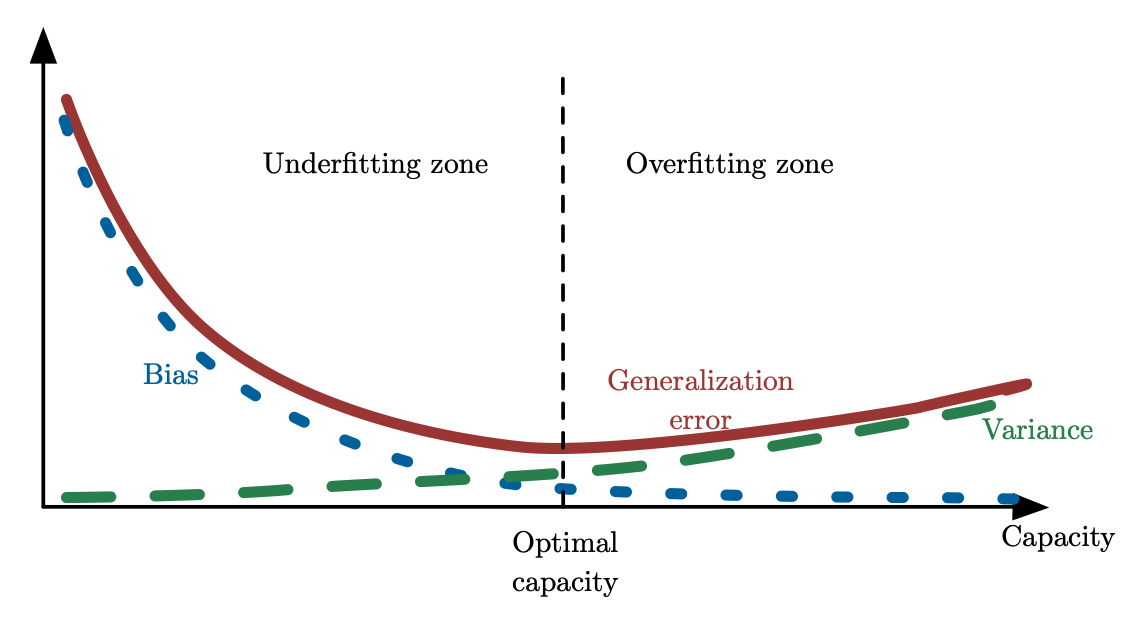
\includegraphics[width=\textwidth]{figs/Bias-Variance.png}
    \caption{با افزایش ظرفیت (محور افقی)، بایاس (نقطه‌چین) کاهش یافته و واریانس (خط‌چین) افزایش می‌یابد. در این صورت خطای تعمیم به فرم یک منحنی $\text{\begin{latin}
        U
    \end{latin}}$ شکل در می‌آید. پس می‌توان ادعا کرد که یک ظرفیت بهینه وجود دارد به گونه‌ای که اگر مقدار آن را کاهش دهیم کم‌برازش، و اگر مقدار آن را افزایش دهیم بیش‌برازش رخ دهد.}
    \label{fig:Bias_Var}
\end{figure}


\subsection{تجزیه بایاس و واریانس}

تجزیه بایاس و واریانس روشی برای تجزیه و تحلیل خطای تعمیم مورد انتظار الگوریتم یادگیری با توجه به یک مسئله خاص به عنوان مجموع سه عبارت، بایاس، واریانس و کمیتی به نام خطای کاهش ناپذیر است که ناشی از نویز موجود در مجموعه داده‌های آموزش حاصل می شود.
در صورتی که در داده‌های آموزش نویزی نداشته باشتیم
می‌توانیم میانگین مربعات خطای یک مدل را به صورت زیر بنویسیم:
 $$\text{\begin{latin}MSE\end{latin}} = \mathbb{E}\left[(\hat{\theta} - \theta)^2 \right] = \text{\begin{latin}Bias\end{latin}}(\hat{\theta})^2 + \text{\begin{latin}Var
 \end{latin}}(\hat{\theta})$$
 می‌توانیم این رابطه را تعمیم دهیم. فرض کنید که یک مجموعه از داده‌های آموزش شامل نقاط 
 $x_1, \cdots , x_n$ 
 و مقادیر حقیقی $y_i$ را که منتناظر با $x_i$ها هستند داریم.
 همچنین در نظر بگیرید که داده‌ها توسط تابع $f(x)$ تولید شده باشند و $y = f(x) + \epsilon$ باشد که $\epsilon$ مقداری نویز با میانگین $0$ و واریانس $\sigma^2$ می‌باشد. در این صورت خواهیم داشت:
 \begin{align*}
     \text{\begin{latin}MSE\end{latin}} & = \mathbb{E}\left[(\hat{y} - y)^2\right] \\
     & =  \mathbb{E}\left[(f(x) + \epsilon - y)^2\right] \\ 
     % & = \mathbb{E} \\
     & = \text{\begin{latin}Bias\end{latin}}(\hat{y})^2 + \text{\begin{latin}Var
 \end{latin}}(\hat{y}) + \sigma^2
 \end{align*}   